\documentclass[a4j,10pt, twocolumn]{jarticle} \usepackage[dvipdfmx]{graphicx} \usepackage{amssymb} \usepackage{amsmath}
\usepackage{float}
\usepackage{slashbox}
\usepackage[compact]{titlesec}
%---------------------------------------------------
% ページの設定
%---------------------------------------------------
\setlength{\textwidth}{180truemm}
\setlength{\textheight}{260truemm}
\setlength{\topmargin}{-12.5truemm}
\setlength{\oddsidemargin}{-10.5truemm}
\pagestyle{empty}
\setlength{\headheight}{0truemm}
\setlength{\parindent}{1zw}

\begin{document}
\twocolumn
[
\begin{center}
  {\huge NAISTにて取り組みたい研究について}
\end{center}
\begin{flushright}
\begin{tabular}{ll}
氏名: & 新妻巧朗\\
試験区分: & 情報科学区分\\
希望研究室: & 自然言語処理研究室
\end{tabular}
\end{flushright}
\vspace{1truemm}
]
\section{はじめに}
\subsection{NAISTで取り組みたいこと}
NAISTにて、私が取り組みたい研究テーマは「情報検索システムにて検索質問に合わせた適切なファセットの生成手法について」である。

このファセットとは、図書館情報学における定義で「あるクラスを2以上の異なる区分特性によって区分したときに得られる下位クラスの総体\cite{libdic}」のことを言う。
また、この区分特性とは「ある分類に属する個々のメンバーに共通する性質」のことである。
つまり、このファセットを具体的に説明すれば、共通の性質を抽出することで得られたある区分で検索結果を絞り込むための切り口のことである。
\section{研究の概要}
\subsection{背景・社会的意義}
 現代社会において情報収集をするためには、検索エンジンを利用することは必要不可欠である。
 しかし、検索エンジンを適切に活用できず、目的の情報に至れない場面も多い。
 それは多くの検索エンジンの仕組みが、利用者に対して情報検索能力を要求しているからである。
 これまでも福島らの研究にて情報検索能力は個人差が大きく、能力差によって情報格差が生じていることが調査されてきた\cite{fukushima}。
 こうした課題を解決することで、情報に辿りつけないことで生じる機会損失を減らすことができるのではないかと考えている。
 過去に齋藤らによる教育を通して情報検索能力を向上させる研究\cite{saito}も存在しているが、本研究ではシステムの拡張によって解決するアプローチを考えていく。

 福島らによって言語能力の高さが情報検索能力の高さに関係しているとわかった\cite{fukushima}。
 つまり、言語能力の高低が情報検索において、情報格差を生み出していると考えられる。
 そのため、情報の探索過程で言語能力を要求する場面にて利用者の補助をおこなうシステムを提案したい。
\subsection{提案内容}

 そこで、利用者が入力した検索質問に対して適切なファセットを表示することで、検索質問を検索意図に近づけていくシステム(図1)を提案したい。

 \begin{figure}[ht]
   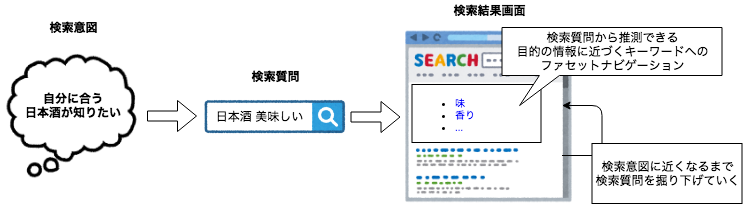
\includegraphics[width=85mm]{./new_ir_with_navi.png}
   \caption{システムのイメージ図}
 \end{figure}
 
 検索意図とは、人が検索行動をおこなう動機のことである。
 情報の探索行動は、検索意図から生じる検索質問を検索の動機を満たす文書に近づけるプロセスであると考えられる。
 そのため、ファセット検索が利用できるのではないかと考えた。
 ファセット検索とは、検索システムの利用者に検索対象を何らかの側面で絞り込むファセットを提示し、検索対象を絞り込んでいく検索手法である\cite{faceted}。
 これはシステムの利用者が検索意図を言語化する行動をシステムが代行していると言える。
 そのため、検索エンジンが個人の言語能力に依存している問題にアプローチできると考えている。
\section{研究の方法}
\subsection{従来のファセット検索の課題}
 ファセット検索の典型的な用例として、Amazon.co.jp\cite{amazon}の検索結果画面をあげる。ファセット検索は図2の赤枠で囲われたメニューのように、ある分類に関する検索結果をさらに絞り込む切り口を提供する。
 \begin{figure}[ht]
   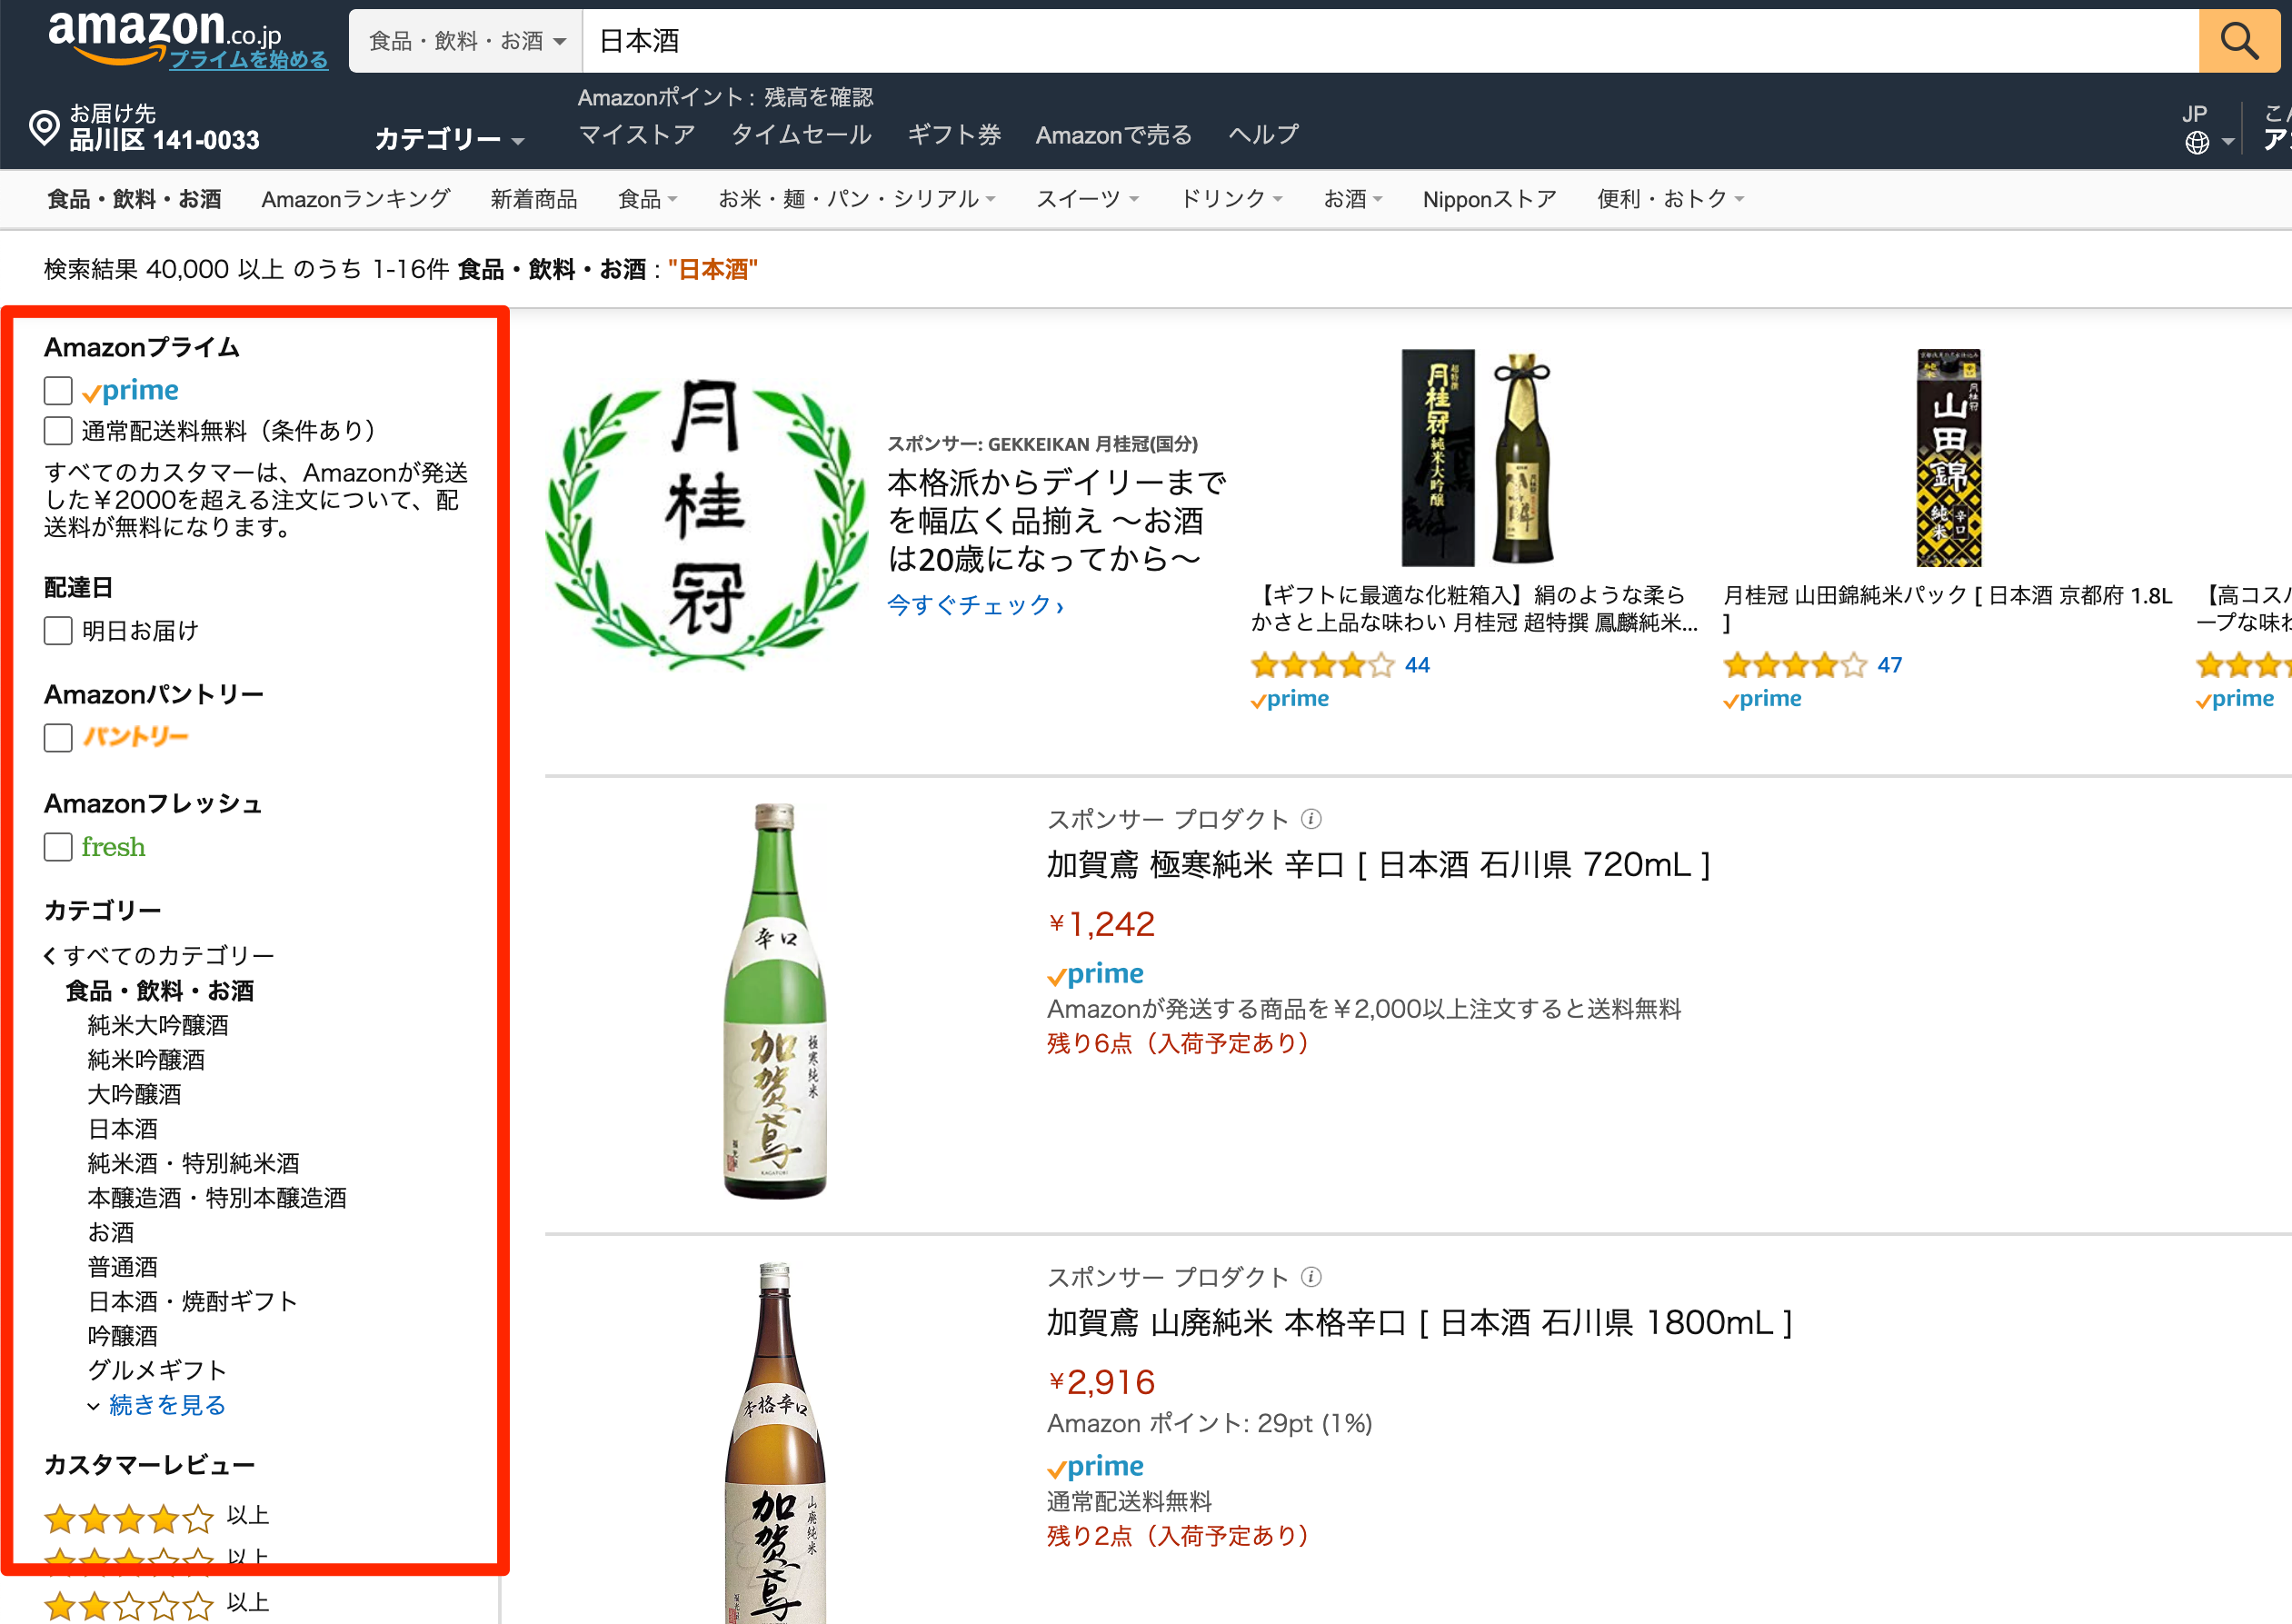
\includegraphics[width=85mm]{./amazon.png}
   \caption{Amazonの検索結果画面: 日本酒に対するファセット検索}
 \end{figure}
  先に挙げた例では、商品データを索引対象として扱っていた。このように従来のファセット検索では、索引対象には既に構造化がされており属性データを持った文書を利用することが多い。
  この属性データとは、ある区分特性に属しているかどうかを示すようなメタデータのことである。

  また、ファセット検索を非構造的な文書にて利用する場合には、事前に文書から区分特性を見つけ出して、それを索引可能な形に変換して属性データとして付与することで半構造的な文書にする必要がある。
  従来であれば、この区分特性を見つけ、属性データの付与する作業は人手を用いておこなわれてきた。しかし、Webを対象にファセットを作成する場合には、文書の増減と文書分類の変化の早さが原因で、人手による作業が現実的でないという課題がある。
  そのため、区分特性を推測し自動的に属性データを生成することで、ファセット検索をWebにも応用できるようにしたいと考えた。

\subsection{研究の方向性}
本システムではファセットを作成するために、二つのデータを出力をすることを目標とする。
\begin{description}
  \item[ファセットを表すtupleのリスト] ある語彙$v$を上位クラスとすると、$v$をある区分特性$c$を介して関係する語彙の集合$V$を下位クラスとして考えるデータからなる$\langle v, c, V\rangle$形式のtupleのリスト。
  \item[属性データ] 文書があるファセットに含まれるかどうかを示す属性データのこと。文書に付与するメタデータとして考える。
\end{description}

\subsubsection{ファセットを表すtupleのリスト}
入力データを索引対象の文書として、教師なしでこのtupleの情報を抽出する方法を考えたい。
区分特性は「関係」をうんちゃらかんちゃらである。そのため、文中の中で語彙の関係を示せる語彙は述語であることから、本システムにおけるは区分特性には述語を利用する。

そのため、区分特性に抽出にはOpenIEと呼ばれる研究の成果を活用できる可能性がある。
OpenIEは文章から$\langle \arg1, rel, \arg2 \rangle$という形式のtupleの形で、情報を抽出をする技術の研究分野である。\cite{niklaus}
この文中の述語を上記のrelとして、その周辺の語彙などをarg1, arg2として抽出する。
このarg1を語彙$v$とrelを区分特性$c$とみなせば、arg1とrelが一致しているtupleが持つarg2を下位クラスの語彙の集合$V$としてまとめることで、$\langle v, c, V\rangle$のtupleを作成できると考えている。

例えば、「日本酒」を語彙$v$とすると、区分特性$c$は「の銘柄は」といった述語となる。そして、その目的語である「一ノ蔵」「花浴陽」などをまとめて、語彙の集合$V$を得れば$\langle "日本酒", "の銘柄は", ["一ノ蔵", "花浴陽", \dots] \rangle$というtupleを作ることができる。

\subsubsection{属性データ}
 3.2.1にて作成したtupleのうち、上位クラスである語彙$v$が文書に関係しているかをブール値で表現するメタデータを文書に付与することで実現できる。tf-idfなどに閾値をもうけて関係性を表現することを検討している。

\subsubsection{まとめ}
 3.2.1のtupleをファセットのユーザインタフェースを作成するのに利用し、検索処理では3.2.2で文書に付与した属性データを利用することで、提案をしたシステムが実現できるのではないかと考えている。

\section{これまでの修学経験等}
 学部では地方の産業構造に関する実証分析について研究してきた。
 特に卒業研究では総生産と地域を構成する産業に着眼し、経済格差が生じる要因について分析をした。
 また、社会人ではソフトウェアエンジニアとしてWebサービスに携わり、検索システムの利用者が得たい情報をどう探索しているのかについて考えてきた。
 特に現在携わっているアルバイト求人のデータベースメディアでは、どのようにファセットナビゲーションを実現するとよいか、求人検索機能のファセット検索をどのように実装すべきかなどを試行錯誤する機会に恵まれた。
 こうした経験が本研究では役立つのではないかと考えている。

\section{最後に}
ここまでNAISTにて取り組みたい研究テーマや自身の経験について述べてきた。
私がNAISTを志望するのは、異なるバックグラウンドを持った人間を受け入れるサポート体制が整っており、かつ優れた研究成果を出している大学院であるからだ。
こうしたNAISTの整った教育・研究環境を活かして、自然言語処理や情報検索の分野に貢献していきたいと考えている。

\begin{thebibliography}{9}
\bibitem{libdic}
  日本図書館情報学会用語辞典編集委員会編 (2013), 図書館情報学用語辞典 第4版
\bibitem{fukushima}
   福島健介・小原 格・須原慎太郎・ほか (2005), インターネット検索能力の差異に及ぼす 要因の検討 その1, コンピュータ&エデュケーション VOL.18 2005
\bibitem{saito}
   齋藤ひとみ・三輪和久 (2004),  Web 情報検索におけるリフレクションの支援, 人工知能学会論文誌 19 巻 4 号 C (2004 年)
\bibitem{faceted}
  Daniel Tunkelang (2009), Faceted Search (Synthesis Lectures on Information Concepts, Retrieval, and Services), pp. 21―26
\bibitem{amazon}
  Amazon.co.jp (最終閲覧日: 2019年5月23日), https://www.amazon.co.jp/
\bibitem{niklaus}
  Christina Niklaus, Matthias Cetto, Andre Freitas, and Siegfried Handschu (2018), A Survey on Open Information Extraction, Proceedings of the 27th International Conference on Computational Linguistics
\end{thebibliography}
\end{document}
